\beginsong{Geburtstagslied}[
    wuw={Aleksander Timofejewski},
    jahr={1971},
    txt={Erik Schellhorn (Übersetzung), letzte Strophe aus studentischen Kreisen},
    txtjahr={1991},
    bo={278}, 
    siru={207}, 
    index={Seht die Leute},
]

\beginverse
\endverse
\centering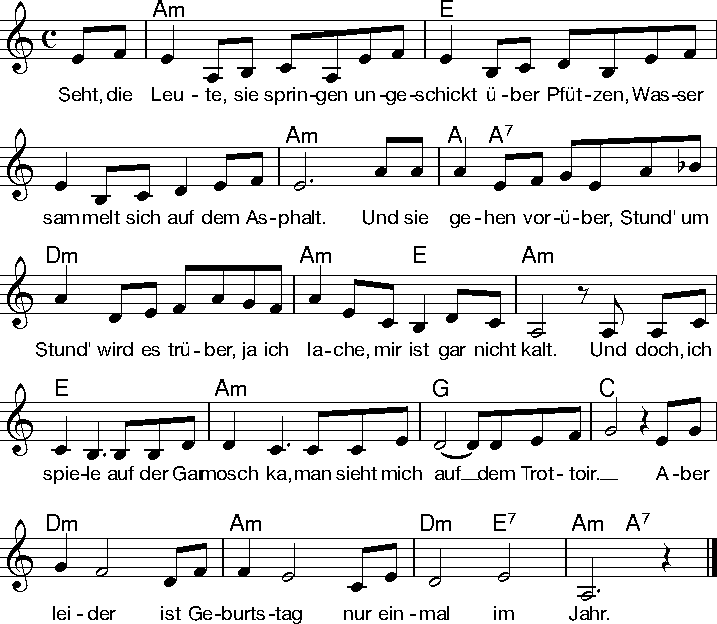
\includegraphics[width=1\textwidth]{Noten/Lied046.pdf}	


\beginverse
Plötzlich \[Am]kommt ein Hubschrauber
und he\[E]raus steigt ein Zaub'rer,
zeigt den Film “Pippi geht auf die \[Am]Walz”.
Zum Ge\[A]burtstag, da wünscht
er mir viel \[Dm]Glück und wie immer
schenkt er \[Am]mir eine \[E]Tonne voll \[Am]Eis.
\endverse

\beginchorus
Und doch, ich \[E]spiele auf der Ga\[Am]moschka,
man sieht mich \[G]auf dem Trotto\[C]ir.
\lrep Aber \[Dm]leider ist Ge\[Am]burtstag
nur ein\[Dm]mal \[E7]im \[Am (A7)]Jahr. \rrep
\endchorus

\beginverse
Ich hab' ^heute Geburtstag,
alle ^kommen am Sonntag,
fröhlich lärmen sie im Haus he^rum.
Und sie ^tanzen, sie singen,
dass die ^Wände mitschwingen,
und zer^stören mein ^Aquari^um.
\endverse

\beginchorus
Oh, wie sie \[E]rauchen und sie ver\[Am]sauen
den Teppich, \[G]der ganz neu noch \[C]war.
\lrep Ach, wie \[Dm]gut, man hat Ge\[Am]burtstag
nur ein\[Dm]mal \[E7]im \[Am (A7)]Jahr. \rrep
\endchorus

\endsong

\beginscripture{}
Dies ist die Übersetzung des ''Liedes des Krokodils Gena'', einer russischen Roman-, Theater- und Zeichentrickfilmfigur.
\endscripture
